\documentclass[cm, 10pt]{article}
% =============================================================== %
%                                                                 %
%                             Packages                            %
%                                                                 %
% =============================================================== %

% Making the page dimensions reasonable
\usepackage[margin=1in, tmargin=1.25in]{geometry}

% For most of the math symbols, and nice things like align
% environment
\usepackage{amsmath, amssymb}

% For \includegraphics
\usepackage{graphicx}

% Fancy page header
\usepackage{fancyhdr}

% For customizing the enumerate environment
\usepackage{enumitem}

% For leftbar environment (for proving lemmas, if needed)
\usepackage{framed}

% For leftbar color
\usepackage{color}

% In case you want any diagrams
% \usepackage{tikz}
% \usetikzlibrary{arrows}
% \usetikzlibrary{arrows.meta}
% \usepackage{pgfplots}
% \usepackage{asymptote}

% ...Which you would probably place in figure environments
% \usepackage{float}

% For referencing page count
\usepackage{lastpage}

% Because I've learned my lesson about manual line breaks
\usepackage{parskip}

% For checkmark
\usepackage{pifont}

% --------------------- Hacky Control Seqs ---------------------- %
% For referencing labeled equations w/ number in parens
\let\oldref\ref
\renewcommand{\ref}[1]{(\oldref{#1})}

% Useful shortcut commands for common sets
\newcommand\CC{{\mathbb C}}
\newcommand\RR{{\mathbb R}}
\newcommand\QQ{{\mathbb Q}}
\newcommand\ZZ{{\mathbb Z}}
\newcommand\NN{{\mathbb N}}

% Commands to avoid exiting math mode
\newcommand{\st}{\text{ st }}
\newcommand{\lub}{\text{lub}}
\newcommand{\glb}{\text{glb}}

% Useful commands for paired delimiters that'll adjust to fit whatever
% argument you pass --> e.g. (<something>), [<something else>]
\newcommand{\set}[1]{\ensuremath{ \left\{ #1 \right\} }}
\newcommand{\pn}[1]{\left( #1 \right)}
\newcommand{\abs}[1]{\left| #1 \right|}
\newcommand{\bk}[1]{\left[ #1 \right]}
\newcommand{\vc}[1]{\left\langle #1 \right\rangle}
\newcommand*\closure[1]{\bar{#1}}

% I use this environment for proving any lemmas I use
\renewenvironment{leftbar}[1][\hsize]
{%
    \def\FrameCommand
    {%
        {\color{black}\vrule width 1.5pt}%
        \hspace{7pt}%
        \fboxsep=\FrameSep%
    }%
    \MakeFramed{\hsize#1\advance\hsize-\width\FrameRestore}%
}%
{\endMakeFramed}

% ----------------------- Header formatting ------------------------ %
\pagestyle{fancy}
\fancyhf{}
\lhead{Name:}
\chead{Homework \# 1}
\rhead{Math 171 - Spring \the\year}
\lfoot{Due Thursday, January 25rd, 2018}
\rfoot{\thepage\ of \pageref{LastPage}}

% I don't like autoindentation for new paragraphs in proofs
\setlength\parindent{0pt}

% Finally, enumerate formatting
\setenumerate[0]{label=(\alph*)}

% =============================================================== %
%                                                                 %
%                             Document                            %
%                                                                 %
% =============================================================== %

\begin{document}

% --------------------------- Problem 1 ---------------------------- %

    % Main document body
    \section*{Problem 2 (Chapter 3.4)}
      Which of the following multiplication tables defined on the set
      $\mathcal{G} = \set{a,b,c,d}$ form a group? Support your answer
      in each case.
      \begin{figure}[h!]
        \centering
        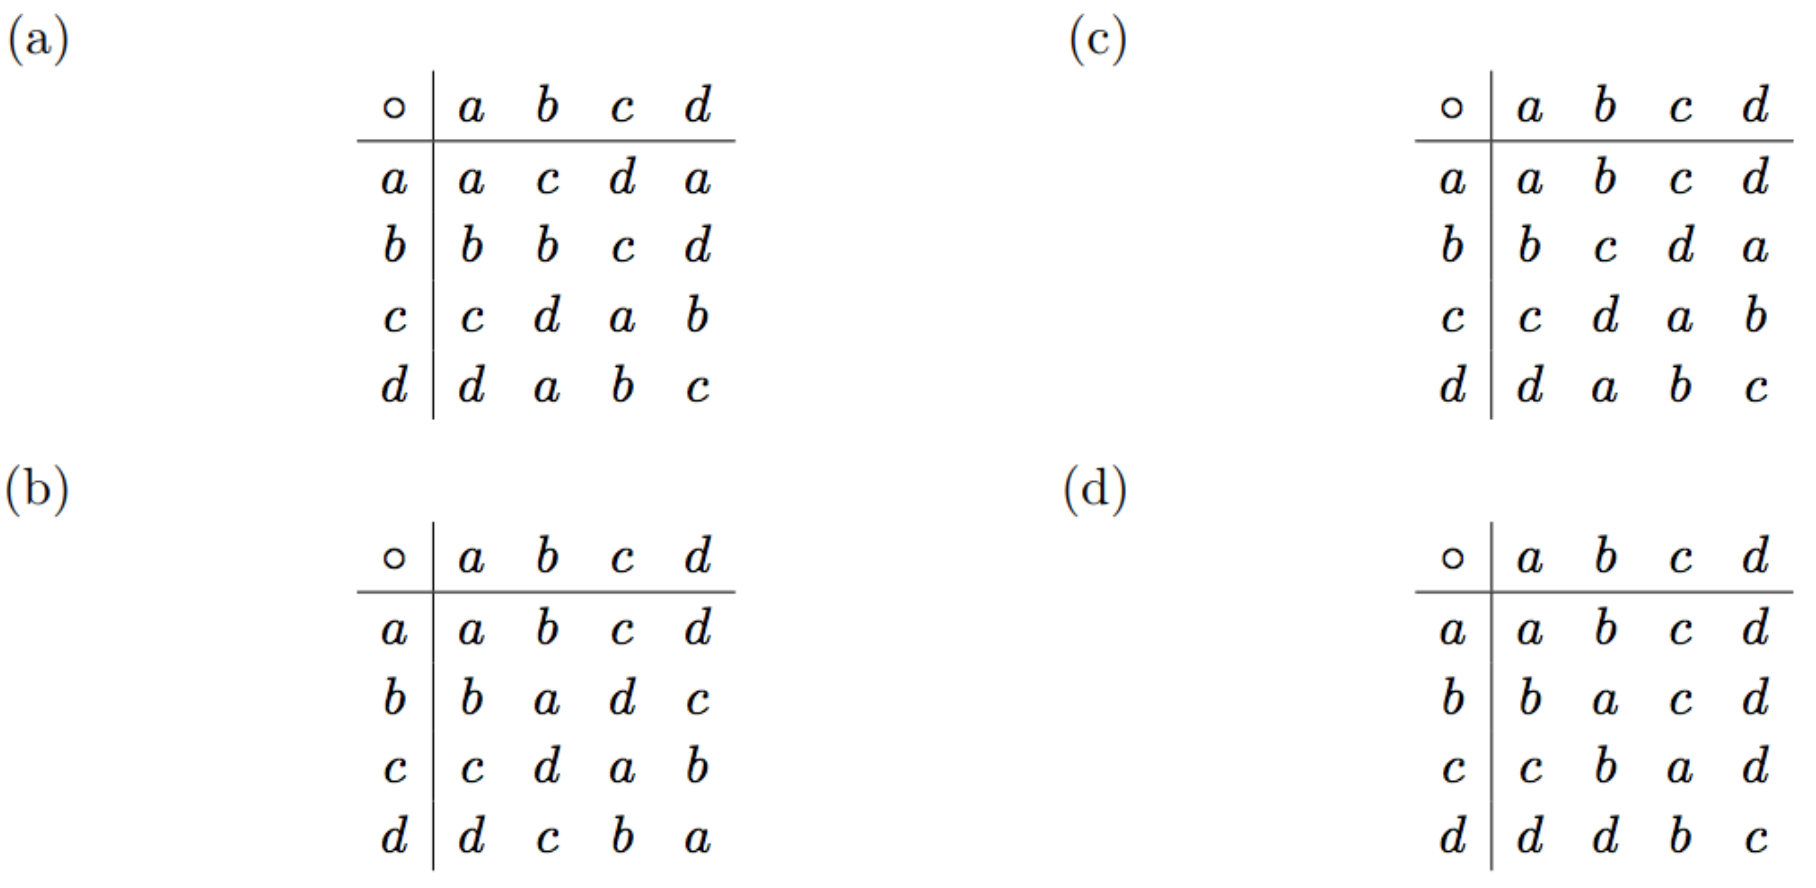
\includegraphics[width=.6\linewidth]{fig1.png}
      \end{figure}

    \hrulefill % fill the line with a horizontal line

    \clearpage % put each problem statement on a fresh page

% --------------------------- Problem 2 ---------------------------- %

    \section*{Problem 5 (Chapter 3.4)}
      Describe the symmetries of a square and prove that the set of
      symmetries is a group. Give a Cayley table for the symmetries.
      How many ways can the vertices of a square be permuted? Is each
      permutation necessarily a symmetry of the square? The symmetry
      group of the square is denoted by $D_4$.

    \hrulefill % fill the line with a horizontal rule

    \clearpage

% --------------------------- Problem 3 ---------------------------- %

    \section*{Problem 10 (Chapter 3.4)}
      Prove that the set of matrices of the form
      \[
        \begin{pmatrix}
          1 & x & y \\
          0 & 1 & z \\
          0 & 0 & 1
        \end{pmatrix}
      \]
      is a group under matrix multiplication. This group, known as the
      \textbf{Heisenberg group}, is important in quantum physics.
      Matrix multiplication in the Heisenberg group is defined by
      \[
        \begin{pmatrix}
          1 & x & y \\
          0 & 1 & z \\
          0 & 0 & 1
        \end{pmatrix}
        \begin{pmatrix}
          1 & x' & y' \\
          0 & 1 & z' \\
          0 & 0 & 1
        \end{pmatrix}
        =
        \begin{pmatrix}
          1 & x + x' & y + y' + xz' \\
          0 & 1 & z + z' \\
          0 & 0 & 1
        \end{pmatrix}.
      \]

    \hrulefill % fill the line with a horizontal rule

    \clearpage

% --------------------------- Problem 4 ---------------------------- %

    \section*{Problem 33 (Chapter 3.4)}
      Let $G$ be a group and suppose that $(ab)^2 = a^2b^2$ for all
      $a$ and $b$ in $G$. Prove that $G$ is an abelian group.

    \hrulefill % fill the line with a horizontal rule

    \clearpage

% --------------------------- Problem 5 ---------------------------- %

    \section*{Problem 48 (Chapter 3.4)}
      Let $G$ be a group and $g \in G$. Show taht
      \[
        Z(G) = \set{x \in G : gx = xg \text{ for all } g \in G}
      \]
      is a subgroup fo $G$. This subgroup is called the
      \textbf{center} of $G$.

    \hrulefill % fill the line with a horizontal rule

    \clearpage

% --------------------------- Problem 6 ---------------------------- %

    \section*{Problem 54 (Chapter 3.4)}
      Let $H$ be a subgroup of $G$. If $g \in G$, show that $gHg^{-1}
      = \set{ghg^{-1} : h \in H}$ is also a subgroup of $G$.

    \hrulefill

\end{document}
